\chapter{A search for new physics in events with a Z boson, missing transverse energy, and jets}

\section{Motivations}

  This is some great motivation!

  \subsection{Motivating Models} \label{sec:susy_models}

  \begin{figure}[h!]
    \centering
    
\includegraphics[width=.5\textwidth]{figures/placeholder.png}
    \caption{\todo{To Be Updated Strong and EWK SUSY diagrams.}}
    \label{fig:SUSY-diagrams}
  \end{figure}

  1. Show the models Strong and EWK SUSY model diagrams we use here.
  2. Discuss why they are useful tools (i.e. give an idea of SMS)

\section{Analysis Strategy}

  \subsection{Background Considerations}

    \subsubsection{Leptonic Final States} \label{sec:leptonic_final_states}
      The Z boson can decay to any fermion. In theory, one could perform this analysis in an all hadronic final state, which might seem advantageous as the Z will decay to hadrons approximately 10 times as often as it will decay to light leptons. \todo{Add some figure for the Z decay rates, probably can site the PDG}. However, there are several reasons leptonic final states are highly advantageous.

      In hadron colliders, the most common types of final states are those with only hadronic activity, as can be seen in figure \ref{fig:lhc_decay_modes}; leptonic final states provide a much cleaner population in which to search for Z bosons. Additionally, as referenced in \ref{sec:electron_measurement_pipeline}, \ref{sec:muon_measurement_pipeline}, and \ref{sec:MET_reco}, the fidelity of energy measurements for the light leptons is much better than for jets at CMS. This provides great advantage for background discrimination; leptons from Z boson decays will tend to have a very specific dilepton mass, a quantity reconstructed from the momentum measurements.

      The decays of the Z produce two opposite sign, same flavor fermions. A further benefit of the leptonic channel is that flavor and charge identification is fairly easy for the light leptons but nearly impossible to identify for jets at the current state of the art (for instance, one can not say with high confidence that a jet was produced by a positively charged charm quark). Finally, the energy and momentum measurements for the light leptons are much better than for jets because of the complexity involved in making good energy measurements for jets. \todo{Point to some discussion about hadron calorimetry, the basic idea here is just that jets have neutral particles and their contribution to the energy measurement needs to be implied by the reconstruction algorithm} 

      Therefore, even though the decay rate to light leptons from Z bosons is lower than the production rate to hadronic final states, the better energy resolution and lower background rate makes the leptonic final state far more powerful.

      When using the leptonic final states, there are essentially two other background sources of leptons we must consider, these are $\gamma$ and W decays. The W boson will decay into leptons only with a complimentary neutrino, this means that in order to select a pair of opposite charge and same flavor leptons, there must be at least two W bosons in the event. Because the decays of the W will be independent, there is only a 50\% chance that the two leptons in an event where two Ws decay leptonically will have the same flavor. As will be discussed later, this makes the background prediction for these types of events very easy as events with two same flavor leptons can be used to model essentially any kinematical distribution.

      Depending on the source of the Ws, the kinematics of the leptons will differ. However, a general rule is that the total energy in the event will be peaked at some low value, near the threshold to produce the event, essentially the sum of the mass of all the prompt particles, and decay exponentially from there. Many kinematic distributions are highly correlated with the total energy in the event. In the case of the Z decay, we know the dilepton mass distribution will not be correlated

      It turns out the most common source of W bosons is through the production of two top quarks, which decay to a bottom quark and a W Boson. To reject these events, we will use B-tagging, described in \todo{add reference to b-tagging section}. Further, the dilepton mass in these events will be essentially random \todo{Add a figure of WW and TTBar production MLL plot for ZMET. Is the distribution flat or falling?} but biased towards lower values. 

      less likely, whereas for Z decay, the breit-wigner distribution predisposes the dilepton mass to be near 91 GeV. 

      The overall dilepton mass distribution will be a falling distribution with a small bump for the Z Boson. 

      \todo{Need to close this off with a discussion about how the backgrounds are mainly DY, TTBar, and VZ}

      Finally, due to the instability of the $\tau$ lepton, we neglect this channel from the search. $\tau$ leptons are much harder to identify than the light leptons, and further they can decay to light leptons in a flavor symmetric manner, so are predicted by that background channel's prediction method.

    \subsubsection{Hadronic Activity Requirements}
      As mentioned above, the major production mode of opposite sign dilepton pairs with dilepton mass near 91 GeV is from Drell-Yan production of Z. The diagram for this type of process is shown in \ref{fig:DY-diagram}. As can be seen in the figure, the leading order diagram for this process has no free quarks or gluons. That there are no free colored particles means that the vast majority of these events will likewise come without any jets. Diagrams with ISR and FSR which take a cross-section production hit of roughly 1/5 \todo{explain this}, which means that we can suppress the DY background by a factor of 100 by requiring at least 2 jets in an event. This keeps our signal count low. Further, the prediction of 0 or 1 jet bins is a completely different process due to the sources of MET, and many of our motivating models will have many jets as part of their decay chain. 

      \begin{figure}[h!]
        \centering
        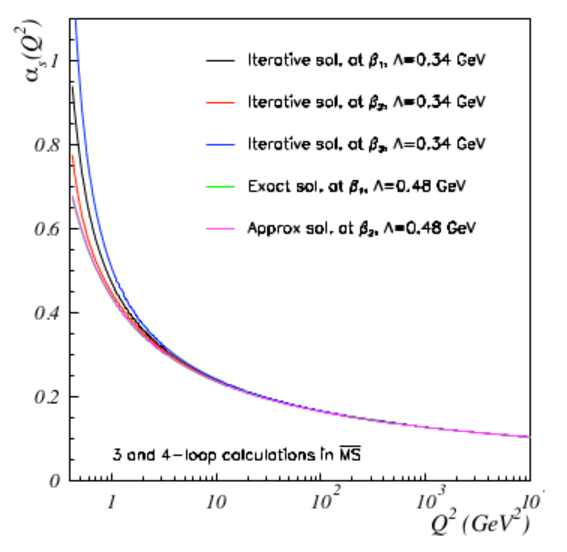
\includegraphics[width=.5\textwidth]{figures/QCD_Coupling_Running.pdf}
        \caption{The QCD coupling constant computed to different orders and different cutoff scales. The production of the Z boson is much more likely at center of mass energy near the mass of the Z. This means that $\alpha_s$ is between $\frac{1}{5}$ and $\frac{1}{10}$, which can be viewed as the zeroth order multiplicative correction to the DY with a single ISR or FSR jet cross section} 
        \label{fig:alpha_s_running}
      \end{figure}

      In fact, strongly produced SUSY models described in \ref{sec:susy_models} anticipate lots of hadronic activity. Therefore, in search regions targeted at those models, we also also ask for lots of hadronic activity by selecting events with high $H_T$, the scalar sum of transverse energy for all jets in an event, above certain thresholds. This further rejects DY events.

      \begin{figure}[h!]
        \centering
        
\includegraphics[width=.5\textwidth]{figures/placeholder.png}
        \caption{\todo{To Be Updated with DY figure.}}
        \label{fig:DY-diagram}
      \end{figure}

    \subsubsection{MET Binning}
      Again, inspecting the diagram above, when the Z decays to charged leptons, no neutrinos are produced. This means that DY has no genuine MET, any missing energy must come from mismeasurements of the jet energy, misattributions of jets to the DY vertex, or loss of objects out of the detectors fiducial area. These should be relatively small effects and we will discuss how we predict the MET distribution for this type of event in the following sections. For now, consider that the leading background when searching for Z bosons can be reduced dramatically by considering only events with high MET. In this analysis, we only look at events with more than 100 GeV of missing energy.

    \subsubsection{MT2}
      The MT2 variable is defined as

      \[
      \min\max{whatever}
      \]

      When a pair of W bosons decay into a lepton and a neutrino, we can see that this value should not be able to be larger than the mass of the W boson, since by summing over all possibilities, we will get the true values which makes the outer minimum select at most the mass of the W (there is no lower limit). However, in the case of an arbitrary decay, for instance in DY or in signal models with dark matter, there is no need for this value to be smaller than the mass of the W and generally higher values will be found. Therefore, we can use this quantity as a handle for rejecting events where the leptons come from two W bosons. We require in our signal regions that MT2 be at least greater than 80 GeV, near the mass of the W boson. This mainly rejects the TTBar background. \todo{Why does any TTBar actually get through?}

    \subsubsection{B-Tagging}
      We also like to bin in b-tags. This is because the background composition changes dramatically with b-tagging as the second largest background is TTBar. This allows us to use a slightly higher MT2 cut in regions with a b-tag, as they will be more dominated by TTBar than by DY since DY is likely not going to have a b-tag even though it might.

\section{Object Selection}

  After the particle flow algorithm identifies lepton, jet, and photon candidates, and before events can be classified as belonging to the various search, control, and closure regions, an additional set of selections are applied in order to further purify the analysis object collection. The purpose of this section is to define these selections, sometimes called a ``preselection."

  \subsection{Lepton ID}
    There are essentially two ways to get ``fake" leptons in the lepton population:

    \begin{enumerate}
      \item A set of calorimeter and tracker hits from hadronic activity mimics the geometry expected by an lepton closely enough that a lepton is reconstructed from what should be called a jet.
      \item An unstable particle, normally a charm or bottom quark, decays via a(n), often virtual, W boson and emits a real lepton and its complimentary neutrino. In physics parlance, this is called \emph{non-prompt} lepton, as it is a secondary decay (\emph{prompt} meaning created at the primary vertex).
    \end{enumerate}

    Although item (2) is a ``real" lepton in the colloquial sense, in the context of most analyses, this one included, we do not want these sorts of objects contaminating our lepton population. To guard against these fake leptons, an additional set of cuts, called an ID is required to be passed by each candidate before it is considered a ``good" lepton.

    In this analysis, we identify two ``working points" for leptons, tight and loose. These categories are defined based the lepton flavor and a set of cuts described below. Any lepton which passes the criteria to be classified as tight would necessarily pass the criteria to be classified as loose.

  \subsection{Lepton Isolation}
    In addition to the ID, isolation requirements are also necessary for leptons to be added to the analysis selection. In this analysis we use the variable miniRelIso, which is defined as the energy inside a variable size cone, determined by the lepton candidates \pt, about the lepton divided by the leptons \pt. The cone size is set by \pt in the following manner (units in \GeV):

    \[   
      \Delta R = 
      \begin{cases}
        0.2                & \pt < 50  \\
        \frac{10}{\pt}     & 50 \le \pt < 200 \\
        0.05               & \pt \ge 200 \\
      \end{cases}.
    \]

    The miniRelIso variable is then defined as the energy of all particle flow candidates inside the cone of size $\Delta R$ with effective area corrections applied \todo{cite EA corrections} divided by the \pt of the lepton.

    \[
      \text{miniRelIso} = \frac{\text{E}_\text{cone}}{\pt}.
    \]


  \subsection{Electron ID and Isolation} \label{sec:electron_id_and_isolation}
    \todo{cite https://arxiv.org/pdf/1502.02701.pdf}
    The electron candidates are required to pass the following cuts in addition to the particle flow identification:

    \begin{table}[!h]
      \begin{center}
      \caption{\label{table:electrons} Requirements for electron identification in addition to particle flow. Variables can be looked up in the \hyperref[ch:glossary]{Glossary} }
        \begin{tabular}{l|c}
          \hline
          Cut variable                  & Requirement   \\
          \hline
          \pt\                           & $>10$ GeV    \\ 
          $d_{0}$ (w.r.t. 1st good PV)   & $<0.05$ cm   \\
          $d_{z}$ (w.r.t. 1st good PV)   & $<0.1$  cm   \\
          miniRelIso / \pt               & $<0.10$      \\
          abs(SIP3D)                     & $< 8$        \\
          maxLostHits                    & $==$ 0       \\
          Conversion Veto                & must pass    \\
          Spring 2016 POG MVA            & see below    \\
          miniRelIso                     & $<0.10$      \\
          \hline
        \end{tabular}
      \end{center}
    \end{table}

    The tight and loose criteria for electrons is based entirely on the MVA output. The POG MVA is a boosted decision tree (BDT)\footnote{A boosted decision tree is a sort of classifier that assigns a real number to a well-formed tuple of data. The algorithm tries to construct a map such that the number output for tuples in the same category are close to each other, then that number can be used discriminate between categories. Technical details are beyond the scope of this thesis, but a good review can be found \todo{find BDT document}. In the case of the electron ID MVA, the categories are real or fake and the numbers lie between -1 and 1.} prepared by the CMS EGamma Physics Object Group (POG). The BDT is trained on simulated Z$\to e^+ e^-$ events where electrons are considered to be real if the candidate can be matched to an electron emitted from the Z, and fake otherwise. An additional validation sample of mostly real electrons in data is constructed from $e^+ e^-$ events where the dilepton mass is within 7.5 GeV of the Z pole mass, $\abs{M_{ll} - M_Z} < 7.5$ GeV, and each lepton is required to be isolated such that the energy in a cone around the electron must be less than 10\% of the total energy in the cone (including the electron). A sample of mostly fake leptons in data is constructed by requiring a third lepton candidate in these events which has inverted isolation criteria and the additional requirement that the MET in the event is less than 25 GeV to suppress WZ events. 

    Distributions of various kinematical quantities are constructed from simulation and data that have reason to discriminate between real and fake electrons, for instance the spread of the calorimeter hits in $\eta$. Some of these distributions are shown in figure \ref{fig:electron_mva_discriminating_vars}. The MVA is trained on the simulated events then checked against the data samples described above for consistency. Finally electrons in the barrel region and endcap regions are partitioned and each set is used to train an MVA specifically targeting the detector subsystems there \cite{cms_electron_photon_performance}. 

    \begin{figure}[!h]
      \centering
      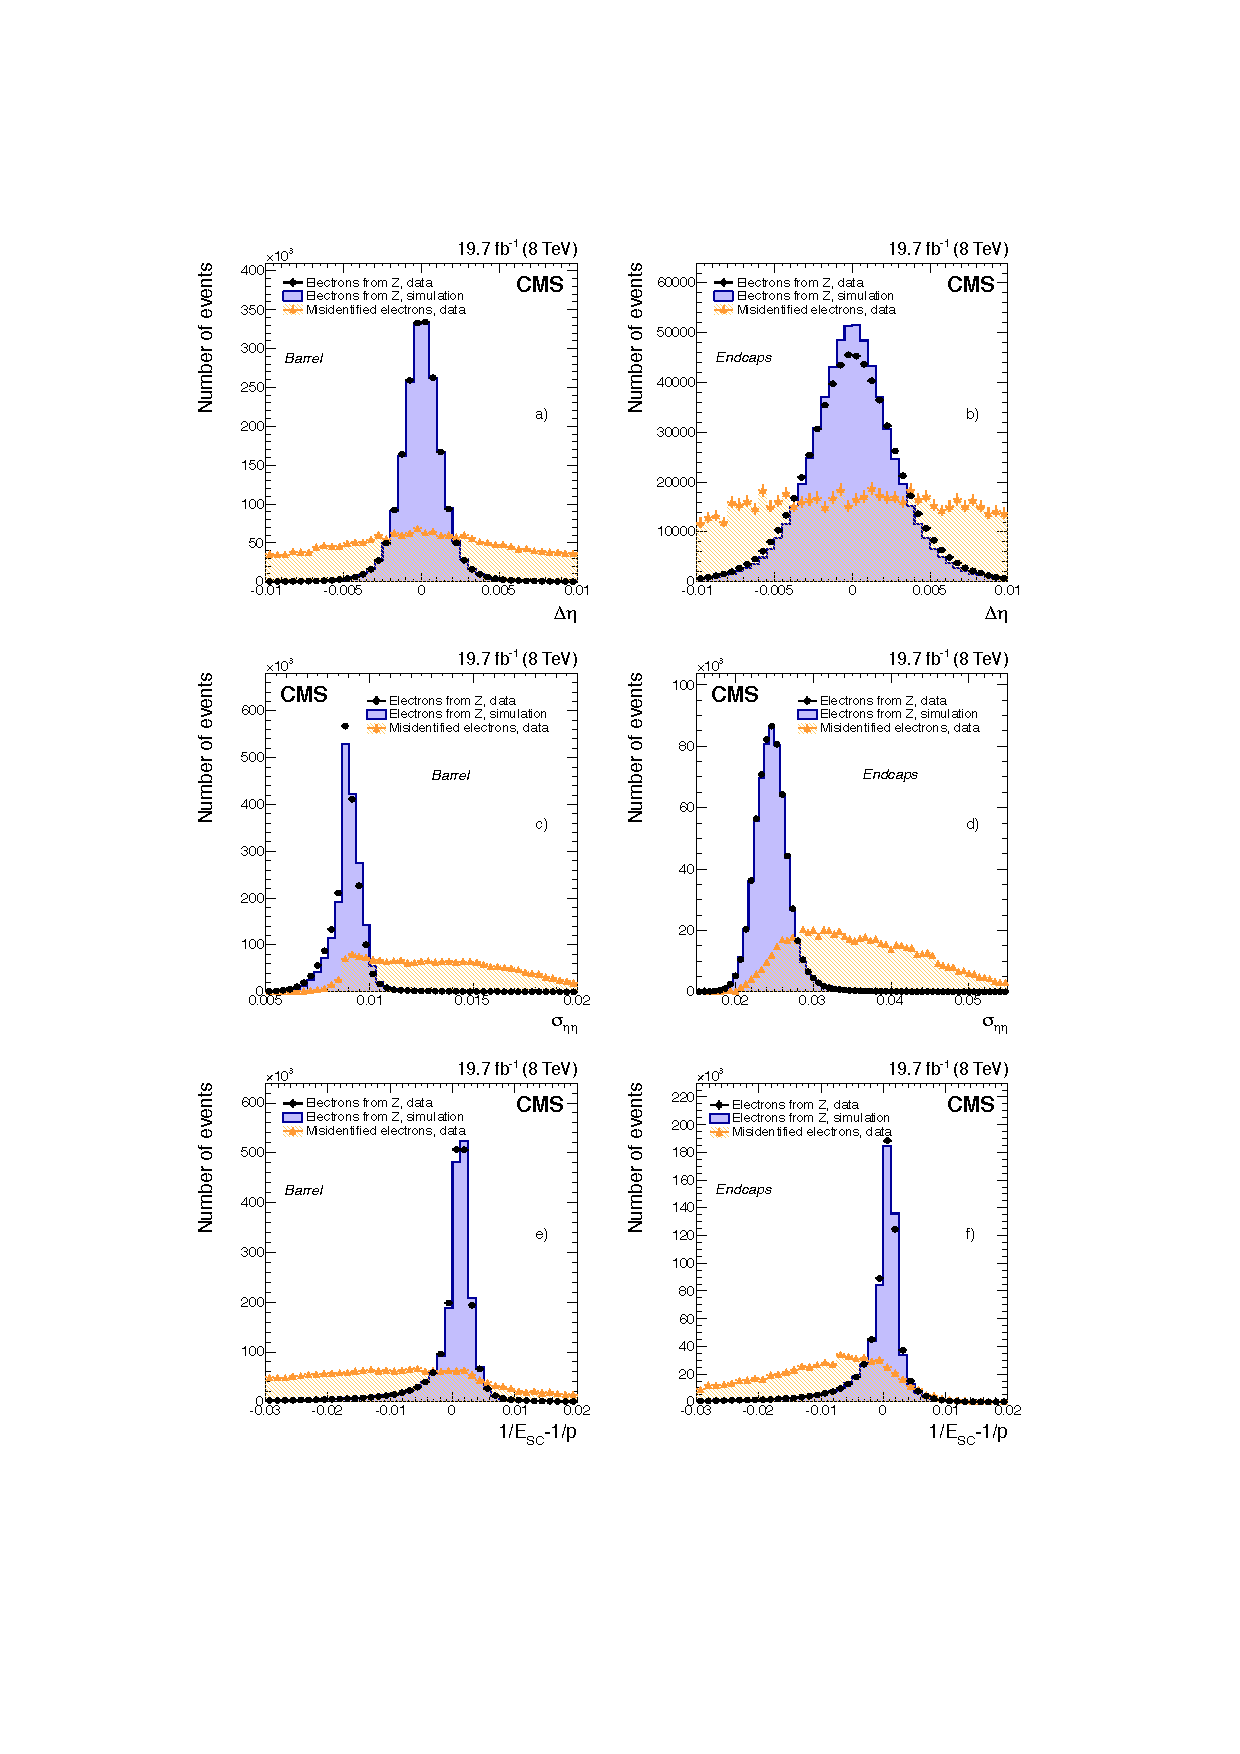
\includegraphics[width=.8\textwidth]{figures/electron_mva_discriminating_distributions.pdf}
      \caption{Some distributions used in the electron MVA that help discriminate between real (prompt) and fake (non-prompt) electrons. Simulation provides a guaranteed way to tag electrons as prompt or not-prompt, and so is used to train the MVA. However, it is important that data and simulation agree in these variables. $\Delta \eta$ and $\sigma_{\eta\eta}$ are variables that characterize the spread of detector hits associated with the electron in the $\eta$ direction. $E_\text{SC}$ is all the energy deposited into the ECAL which is associated to the electron, and $p$ is the electron's momentum. \todo{Do I need to make these plots myself?}}
      \label{fig:electron_mva_discriminating_vars}
    \end{figure}

    The working points for electrons based on the MVA output are shown below:

    \begin{table}[!h]
      \begin{center}
        \caption{\label{tab:elId}  Electron identification working points used in this analysis.}
        \begin{tabular}{rl|rl|l|l}
          \hline
          \multicolumn{2}{c|}{pseudorapidity region} & \multicolumn{2}{c|}{momentum [GeV]} & loose WP & tight WP \\ 
          \hline\hline
          $0<~|\eta|$&$<0.8$     &  10 $<$ ~\pt\ &$<$ 15 &  -0.86 & 0.77 \\ 
          $0<~|\eta|$&$<0.8$     &  15 $<$ ~\pt\ &$<$ 25 &  -0.96+$0.10*\frac{\pt-15}{10}$ & 0.52+$0.25*\frac{\pt-15}{10}$ \\ 
          $0<~|\eta|$&$<0.8$     &   ~\pt\ &$>$ 25       &  -0.96 & 0.52 \\ 
          \hline
          $0.8<~|\eta|$&$<1.479$ &  10 $<$ ~\pt\ &$<$ 15 &  -0.85 & 0.56 \\ 
          $0.8<~|\eta|$&$<1.479$ &  15 $<$ ~\pt\ &$<$ 25 &  -0.96+$0.11*\frac{\pt-15}{10}$ & 0.11+$0.45*\frac{\pt-15}{10}$ \\ 
          $0.8<~|\eta|$&$<1.479$ &   ~\pt\ &$>$ 25       &  -0.96 & 0.11 \\ 
          \hline
          $1.479<~|\eta|$&$<2.5$ &  10 $<$ ~\pt\ &$<$ 15 &  -0.81 & 0.48 \\ 
          $1.479<~|\eta|$&$<2.5$ &  15 $<$ ~\pt\ &$<$ 25 &  -0.95+$0.14*\frac{\pt-15}{10}$ & -0.01+$0.49*\frac{\pt-15}{10}$ \\ 
          $1.479<~|\eta|$&$<2.5$ &  ~\pt\ &$>$ 25        &  -0.95 & -0.01 \\ 
          \hline\hline
        \end{tabular}
        
      \end{center}
    \end{table}

  \subsection{Muon ID and Isolation} \label{sec:muon_id_and_isolation}

    The muon ID is based purely on a cut-based approach, no MVA is used. Again, the selection criteria is based upon the muon POG, which is documented in more detail at ~\cite{muon_POG}. The selection used for the muon ID and isolation are defined below:

    \begin{table}[!h]
      \begin{center}
        \caption{\label{table:muons} Summary of the muons selection requirements. \todo{Version from Bobak's Thesis} }
        \begin{tabular}{l|c|c}
          \hline
          \hline
          \multicolumn{3}{c}{Good Global Muon Requirements} \\
          \hline
          Quantity   &  Tight Requirement & Loose Requirement \\
          \hline
          Fraction of valid tracker hits    & $>$ 0.8     & $>$ 0.8  \\ 
          Normalized global-track $\chi^2$  & $<$ 3       & $<$ 3    \\
          Tracker-Standalone position match & $<$ 12      & $<$ 12   \\
          Kick finder                       & $<$ 20      & $<$ 20   \\
          Segment compatibility             &$>$ 0.451 or & $>$ 0.303 \\
                                            &passes above requirements & \\
          \hline
          muon type & \multicolumn{2}{c}{(global muon or tracker muon) and PF muon} \\
          \hline
          $d_{0}$ (w.r.t. 1st good PV)   & $<0.05$ cm & $<0.05$ cm \\
          $d_{z}$ (w.r.t. 1st good PV)   & $<0.1$ cm  & $<0.1$ cm  \\
          SIP3D                          & $< 8$      & $< 8$      \\
          miniRelIso                     & $<0.20$ & $<0.40$       \\
          \hline
        \end{tabular}
      \end{center}
    \end{table}

    \todo{brief blurb on global/tracker muons.}

\newpage

  \subsection{Photon Selection} \label{sec:photon_selection}

    Photons are used in this analysis as part of the Z+Hadronic background prediction. The details of this prediction are in \ref{sec:z_+_hadronic}

    \begin{itemize}
      \item \pt $ > 22$ GeV
      \item $|\eta| < 2.4$
      \item No matching pixel track (pixel veto)
      \item There must be a jet candidate of \pt $ >$ 10 GeV matched to the photon within $\mathrm{ \Delta R} < 0.3$. 
      The matched jet is required to have a neutral electromagnetic energy fraction of at least 70\%.

      \item We reject photons which have an electron of at least \pt $>$ 10 GeV within $\mathrm{ \Delta R} < 0.2$
      in order to reject conversions from electrons from W decays which are accompanied by real MET.

      \item We reject photons which are aligned with the MET to within 0.4 radians in phi.
      \item To ensure full efficiency with respect to the isolated photon triggers used, we apply the following additional cuts:
      \begin{itemize}
        \item ratio of the energy of the energy of the photon's 3X3 supercluster to the photons 5X5 supercluster (R9) $>$ 0.92
        \item $\frac{H}{E} < 0.2$ %\fixme{is this the HLT H/E or still offline?}
        \item hollow track isolation $<$ 3 GeV
        \item photons with $|\eta| < 1.4$ have ECAL pfcluster iso $<$ 3 GeV + \pt ($\gamma$) * 0.0053
        \item photons with $|\eta| < 1.4$ have HCAL pfcluster iso $<$ 7 GeV + \pt ($\gamma$) * 0.014
        \item photons with $|\eta| > 1.6$ have ECAL pfcluster iso $<$ 3 GeV + \pt ($\gamma$) * 0.0034
        \item photons with $|\eta| > 1.6$ have HCAL pfcluster iso $<$ 7 GeV + \pt ($\gamma$) * 0.0139
      \end{itemize}
    \end{itemize}

  \subsection{Jet Selection} \label{sec:jet_selection}

  \subsection{Isolated Tracks} \label{sec:isolated_tracks}

\section{Event Selection}

  The selection of events can be broken into several stages. Though each of these regions will be expanded upon in the following sections, in broad strokes there 4 separate final states used to accomplish this analysis. These final states define the signal regions and 3 control regions used to conduct this search:

  \begin{description}
    \bitem{Search Regions (SR)} Events with two opposite charge and same flavor light leptons build our search regions, we have either a $e^+e^-$ or a $\mu^+ \mu^-$ pair in each event.
    \bitem{Flavor Symmetric Control Regions (FSCR)} Events with two opposite charge and different flavor light leptons build our flavor symmetric control region, we have either a $e^+\mu^-$ or a $\mu^+ e^-$ pair in each event. This region is used to predict the flavor symmetric background.
    \bitem{MET Templates Control Region (MTCR)} Events with a single photon are used to construct the MET templates control region. 
    \bitem{EWK Contamination Closure Region (ECCR)} Events with a photon and muon are used to check the modeling of the ``EWK contamination" in the MET Templates prediction, described in section \ref{sec:ewk_subtraction}.
  \end{description}

  The CMS datasets which seed these events are described in \ref{sec:datasets}.
  
  \subsection{Lepton Selection}
    The following are the requirements for events with two light leptons, i.e. for the search regions and for the FSCR. The requirements for the MTCR and ECCR are described in section \ref{sec:met_templates_control_region} and \ref{sec:ewk_subtraction_closure_region} respectively. 

    Light lepton candidates are tagged by the particle flow algorithm described in section \ref{sec:particle_flow}. In addition to the list below, leptons must also pass preselection ID and isolation requirements which differ depending on their flavor, but are described in \ref{sec:electron_id_and_isolation} and \ref{sec:muon_id_and_isolation} above.

    \begin{itemize}
      \item The (sub)leading lepton in each event must have at least (20) 25 GeV of transverse momentum. These points were selected so that the event would be in the "trigger turn-on" described in \ref{sec:event_triggering}.
      \item The pseudorapidity for each lepton must be within the inner tracker's fiducial area, namely $\left|\eta\right| < 2.4$
      \item For the search region, events must have exactly one pair of opposite charge same flavor (OCSF) light leptons, for the FSCR events must have exactly one pair of opposite charge and different flavor (OCDF) light leptons.
      \item The mass constructed out of the sum of lepton vectors (dilepton mass) must be between 86 and 96 GeV.
      \item The transverse momentum of the dilepton system must be at least 25 GeV in order to ensure the Z+hadronic background prediction has enough statistics. This is explained in more detail in \ref{sec:z_+_hadronic}.
    \end{itemize}

  \subsection{Event Vetos}
    Events are generally vetoed across all search, control, and closure regions if any of the following are true:

    \begin{description}
      \bitem{Isolated Track Veto} Events with an isolated track, defined in \ref{sec:isolated_tracks}.
      \bitem{MET Filters} Events where any of the ``MET Filters", described in section \ref{sec:met_filters}, are true.
    \end{description}

    Dilepton events specifically, those within the SRs and FSCRs, are vetoed under the following conditions:

      \begin{description}
        \bitem{Lepton Cone Isolation} The two tight leptons are within a cone of $\Delta R < 0.1$ of each other.
        \bitem{Extra Lepton Veto} There is an additional loose or tighter lepton in the event. In other words, event with three or more loose IDed leptons are vetoed. IDs are defined in \ref{sec:electron_id_and_isolation} and \ref{sec:muon_id_and_isolation}. 
      \end{description}

  \subsection{Search Regions}
    Electroweak search regions and strong search regions

  \subsection{Flavor Symmetric Control Region} \label{sec:flavor_symmetric_control_region}
    A flavor symmetric control region in constructed for every search region by flipping the requirement for an OCSF dilepton pair to a OCDF dilepton pair. The number of events in these regions is used to predict the background of events where the two leptons come from a pair of W bosons as described in \ref{sec:flavor_symmetric_background}

  \subsection{MET Templates Closure Region} \label{sec:met_templates_control_region}

  \subsection{EWK Subtraction Closure Region} \label{sec:ewk_subtraction_closure_region}



\section{Background Estimation Methods}
  Fakes are taken care of by the flavor symmetric BG.

  For the signal regions, we select events with opposite charge and same flavor dilepton pairs, for the flavor-symmetric background prediction, we select events with same sign and same flavor dilepton pairs, for the MET templates prediction, we select from single photon events which are seeded by an entirely different dataset.

  \subsection{Z + Hadronic} \label{sec:z_+_hadronic}
  PT of the Z greater than 25 GeV for photon trigger.
    
    \subsubsection{Contamination From Events With Real MET (Electroweak Subtraction)} \label{sec:ewk_subtraction}
      Explain the EWK subtraction method here.

    \subsubsection{Electroweak Subtraction Control Region} \ref{sec:ewk_subtraction_control_region}

  \subsection{Flavor Symmetric Background} \label{sec:flavor_symmetric_background}

  \subsection{Z + $\nu$} \label{sec:z_+_neutrino}

\section{Results}

\section{Signal Interpretations} 

\section{The Electroweak Combination}

The things we want to consider here are: 

  1. All the cuts and stuff, I want to list out what cuts we made and why we chose them. I am not sure where I will put all the data/MC agreement stuff. I guess that's mostly important for the MET profile as I don't really use MC in the rest of the
